\chapter{Predchádzajúce riešenia}\label{chap:previous_solutions}

Problematika peny a bublín zaujala mnohých matematikov, fyzikov a taktiež vedcov v oblasti IT. Skúmanie ich fyzikálnych vlastností má svoje počiatky už v 19. storočí. Ako prvý sa o vysvetlenie tohto fyzikálneho javu pokúšal belgický fyzik Joseph Antoine Ferdinand Plateau. V roku 1873 v práci „Statique Expérimentale et Théorique des Liquides soumis aux seules Forces Meléculaires“ \cite{plateau1873} popísal pravidlá známe ako „Plateauové pravidlá“, ktoré popisujú štruktúru filmov bublín a zabezpečujú štruktúru suchej peny, ktorá minimalizuje povrch bublín v závislosti od ich veľkostí. Sú to tieto pravidlá:

\begin{enumerate}
  \item Tri hladké povrchy mydlových filmov sa pretínajú pozdĺž priamky.
  \item Uhol medzi ktorýmikoľvek dvoma dotykovými rovinami k pretínajúcim sa povrchom, je v každom bode priamky, pozdĺž ktorej sa pretínajú tri povrchy, 120º.
  \item V jednom bode sa môžu spojiť maximálne 4 hrany, z ktorých každá z nich je tvorená priesečníkom troch povrchov a spolu tvoria štvorboký uhol 190º 28’ 16’’ medzi každými dvoma susednými hranami.
\end{enumerate}

Takmer o storočie neskôr, v roku 1976, Taylor \cite{taylor1976} dokázal, že táto štruktúra naozaj minimalizuje povrch bublín. Na rozdiel od suchej peny, mokrá pena má zložitejšiu štruktúru kôli väčšiemu obsahu tekutiny. Takýto typ peny bol takisto skúmaný, a to konkrétne tímami Weaire a spol. \cite{weaire1993} v roku 1993, Herzhaft a spol. \cite{herzhaft2005} v roku 2005 a Piazza a spol. \cite{piazza2008} v roku 2008. Štruktúra peny sa však dá klasifikovať aj na základe veľkosti bublín, tzv. monodisperzná pena, ktorá je tvorená bublinami rovnakej veľkosti \cite{kraynik2003}, alebo naopak polydisperzná, ktorá je tvorená bublinami rôznych veľkostí \cite{kraynik2004}. Vďaka podobnosti váženého Voronoivho diagramu s geometriou peny vedci skúmali využitie takéhoto diagramu na modelovanie statickej peny \cite{redenbach2012}.

Z hľadiska simulácie peny treba brať do úvahy dva aspekty: deformácia jednotlivých bublín a interakcia medzi bublinami navzájom a medzi bublinami a tekutinou, resp. tuhým telesom. O prvý pokus simulácie zohľadňujúcej deformáciu bublín sa zaslúžil Brakke \cite{brakke1992} v roku 1992. Ďurikovič \cite{durikovic2001} v roku 2001 použil na reprezentáciu povrchu bublín mesh (sieť) a interakčné sily aproximoval použitím intermolekulárneho Van der Wallovho modelu síl. Hong a spol. \cite{hong2003} v roku 2003 a Mihalef a spol. \cite{mihalef2006} v roku 2006 ukázali, že na simulovanie deformovateľných bublín možno použiť takisto implicitnú reprezentáciu ako je napr. VOF (Volume-of-Fluid). Zheng a spol. \cite{zheng2006} v roku 2006 navrhli metódu využívajúcu množinu na regionálnej úrovni, pomocou ktorej implicitne modelujú penu ako multimanifoldný povrch. V roku 2007 Kim a spol. \cite{kim2007} pridali do tejto metódy stratu objemu pomocou techniky na ovládanie objemu. Keďže tieto metódy zohľadňujú deformáciu jednotlivých bublín, odzrkadľuje sa to na výpočtovej náročnosti pri väčšom množstve bublín. Ignorujúc deformáciu povrchu bublín, existujú simulácie založené na princípe časticových systémov, ktoré zohľadňujú interakciu bublín s prostredím, avšak bubliny sa nedeformujú a ich priesečníky sú často aproximované. Durian \cite{durian1995} v roku 1995 ako prvý navrhol na animáciu interakcií bublín v 2D pružinový systém. Kück a spol. \cite{kueck2002} v roku 2002 rozšírili túto myšlienku do 3D a takisto našli spôsob ako renderovať Plateauove okraje a zaoblené filmy medzi dvoma dotýkajúcimi sa bublinami. Greenwood a House \cite{greenwood2004} v roku 2004 začlenili Kückov model do simulátora tekutín založeného na časticovom systéme na úrovni množín. V tom istom roku vedci s MPI \cite{sunkel2004} využili vo svojom modeli na simuláciu a renderovanie programy zbiehajúce na GPU, tzv. shadre. Interakcie bublín sa dajú aproximovať takisto pomocou SPH tak ako to spravili Cleary a spol. \cite{cleary2007} v roku 2007, Thürey a spol. \cite{thurey2007} v roku 2007 a Hong a spol. \cite{hong2008} v roku 2008. Nakoniec v roku 2012 navrhli model na simuláciu peny Busaryev a spol. \cite{busaryev2012}, ktorí v tomto modeli využili aj vážený Voronoiov diagram a ich časticový systém dokáže simulovať pohyb bublín s veľkým množstvom za relatívne krátky výpočtový čas.

Ja osobne som sa detailnejšie zaoberal tromi vedeckými článkami, ktoré mi pomohli pri riešení tejto problematiky, a v mojej diplomovej práci som sa inšpiroval konkrétne dvoma z nich. Teraz sa budem venovať trochu podrobnejšie práve týmto článkom a rozoberiem ich prístup a riešenia problematiky peny a jednotlivých bublín. Sú to tieto tri články:

\begin{itemize}
  \item Animation of Soap Bubble Dynamics, Cluster Formation and Collision \cite{durikovic2001}
  \item Rendering and Simulation of Liquid Foams \cite{sunkel2004}
  \item Animating Bubble Interactions in a Liquid Foam \cite{busaryev2012}
\end{itemize}

\section{Animation of Soap Bubble Dynamics, Cluster Formation and Collision \cite{durikovic2001}}

Hlavným cieľom tohto článku je návrh fyzikálneho modelu, ktorý umožňuje simulovať vznik bubliny, deformáciu bubliny, kolíziu bubliny s rovinným povrchom a takisto dynamiku kolízie dvoch bublín navzájom. V článku sú rozobraté jednotlivé zoskupenia medzi bublinami, ktoré môžu nastať pri kolízií bublín, či už zoskupenie dvoch bublín ale aj zoskupenie troch bublín a geometria bublín v týchto zoskupeniach. Ďalej sú v článku podrobne popísané všetky sily, ktoré tento model zohľadňuje. Na záver je v článku popísaná kolízia medzi bublinou a rovinným povrchom.

\subsection{Bubliny}

Bubliny sú v tomto modeli reprezentované pomocou meshu, vďaka čomu tento model umožňuje nepravidelný tvar bublín a tým pádom ich deformáciu. Bublina je povrch s minimálnou energiou svojho druhu tvorený mydlovým filmom. Vo vzťahu k objemu má každá bublina najmenší možný povrch. Pre takto tvorený povrch boli vynájdené spoločné geometrické vlastnosti a tieto vlastnosti sú popísané v hore uvedených Plateauových pravidlách. Mydlová pena pozostáva z množstva bublín rôznych veľkostí, ktorých tvar závisí od prvých dvoch Plateauových pravidiel.

\newpage

\subsection{Zoskupenie dvoch bublín}

Zoskupenie dvoch bublín je tvorené dvoma bublinami, ktoré sa navzájom pretínajú a sú oddelené membránou, ktorá je hranicou ich priesečníku. Takéto zoskupenie minimalizuje plochu filmov bublín. 
\begin{figure}[H]
	\begin{center}
		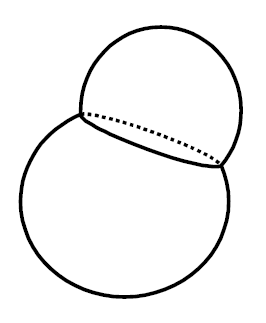
\includegraphics[height=\imageHeight]{images/durikovic/double_bubble}
		\caption{Zoskupenie dvoch bublín \cite{durikovic2001}.}
		\label{img:double_bubble}
	\end{center}
\end{figure}

\noindent Geometria každej z týchto dvoch bublín je tvorená z veľkej časti z guľovitých obalov z mydlových filmov oddelených guľovitou čiapkou tvorenú takisto mydlovým filmom. V prípade, že veľkosť bublín je odlišná, menšia bublina vniká do väčšej, čo je spôsobené väčším vnútorným tlakom v porovnaní s tlakom vo väčšej bubline a tak je ich spoločná stena preliačená smerom do väčšej bubliny. Na obrázku \reference{img:curvature_of_double_bubble_shells} vidieť zoskupenie dvoch bublín s polomermi r\sub{A} a r\sub{B} a s vnútornými tlakmi P\sub{A} a P\sub{B} vyplývajúcich s Plateauových pravidiel, z ktorých tiež vyplýva nasledujúci recipročný vzťah:
\begin{equation}
	\frac{1}{r_{B}} = \frac{1}{r_{A}} + \frac{1}{r_{C}},
\end{equation}
kde r\sub{C} je polomer ich spoločného povrchu.
\begin{figure}[H]
	\begin{center}
		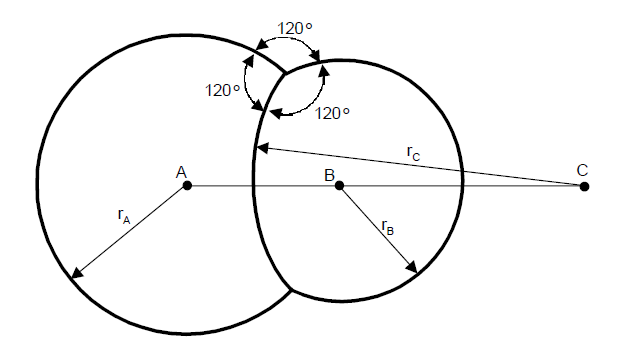
\includegraphics[height=\imageHeight]{images/durikovic/curvature_of_double_bubble_shells}
		\caption{Zaoblenie zoskupenia dvoch bublín \cite{durikovic2001}.}
		\label{img:curvature_of_double_bubble_shells}
	\end{center}
\end{figure}

\subsection{Zoskupenie troch bublín}

Podobne ako pri zoskupení dvoch bublín, aj pri zoskupení troch bublín sa všetky tri guľovité povrchy stretávajú pod uhlom 120º. Stredy zaoblenia troch bublín A, B, D a ich troch spoločných stien, ležia nevyhnutne v jednej rovine. Takisto stredy zaoblenia troch spoločných stien C, E a F ležia nevyhnutne na jednej priamke. Rovnica 1 platí pre každý pár bublín v tomto zoskupení a tak dostávame ďalšie dva recipročné vzťahy:
\begin{equation}
	\frac{1}{r_{D}} = \frac{1}{r_{A}} + \frac{1}{r_{E}} \qquad,\qquad \frac{1}{r_{D}} = \frac{1}{r_{B}} + \frac{1}{r_{F}},
\end{equation}
kde polomer tretej bubliny je rD. Dva nové povrchy rozdeľujúce bubliny so stredmi A a D, resp. B a D sú vytvorené a ich polomery sú r\sub{E}, resp. r\sub{F}. Na obrázku \reference{img:curvature_of_tripple_bubble_shells} vidno zaoblenie takéhoto zoskupenia.
\begin{figure}[H]
	\begin{center}
		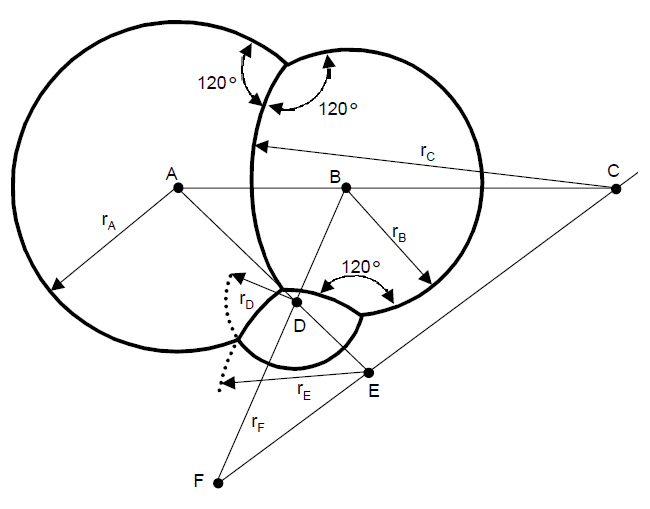
\includegraphics[height=\imageHeight]{images/durikovic/curvature_of_tripple_bubble_shells}
		\caption{Zaoblenie zoskupenia troch bublín \cite{durikovic2001}.}
		\label{img:curvature_of_tripple_bubble_shells}
	\end{center}
\end{figure}

\subsection{Dynamika}

Experimenty ukázali, že bublina, resp. jej mydlový film, je elastický. Preto pri rátaní pohybu bol uvažovaný elastický model od Terzopoulosa a Fleischera. Rovnica pohybu pre elastický deformovateľný model je:
\begin{equation}
	M\frac{\partial^{2} x_{i}}{\partial t^{2}} = F_{i}(t)-\gamma\frac{\partial x_{i}}{\partial t}-\frac{\delta \epsilon (x)}{\delta x_{i}},
\end{equation}
kde x\sub{i} je pozícia častice \textit{i}, \textit{M} je hustota hmoty, \textit{$\gamma$} je konštanta tlmenia, \textit{F\sub{i}(t)} je externe pôsobiaca sila a \textit{$\delta \epsilon$(x)/$\delta$x}  je interná energia, ktorá odoláva deformovaniu bubliny.

\subsection{Pôsobiace sily}

Na bubliny pôsobí výsledná externá sila, ktorá je tvorená súčtom viacerých externých síl ako napr. gravitácia, pretlak, externá kvapalina, odporová sila a interakčné sily.
\begin{equation}
	F_{i}(t)=F_{grav}+F_{excess}+F_{drag}+F_{rep}+F_{lennard}+F_{plane}.	
\end{equation}
\begin{minipage}{\linewidth}
	Na obrázku \reference{img:forces} vidno smer jednotlivých síl pôsobiacich na bublinu.
	\begin{figure}[H]
		\begin{center}
			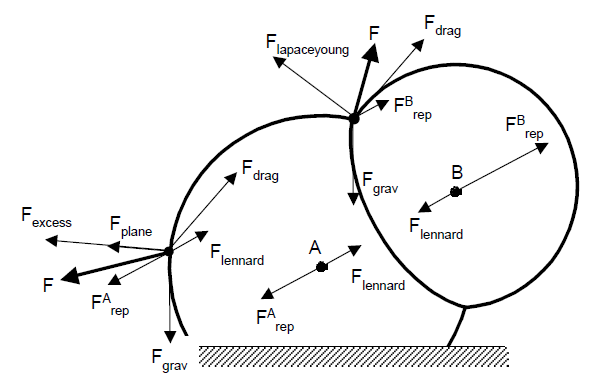
\includegraphics[height=\imageHeight]{images/durikovic/forces}
			\caption{Sily pôsobiace na bublinu \cite{durikovic2001}.}
			\label{img:forces}
		\end{center}
	\end{figure}
\end{minipage}

\subsection{Diskusia}

Pomocou tejto metódy bol vytvorený simulátor bublín, ktorý dokáže interaktívne simulovať bubliny pokiaľ počet bublín nepresiahne šesť. Tento simulátor umožňuje vizualizovať tieto bubliny ako drôtený model, alebo ako jednoduchý OpenGL model. Takisto však podporuje generovanie súborov pre POV-Ray renderer, pomocou ktorého následne môžu byť vyrenderované snímky vo vysokej kvalite.
\begin{figure}[H]
	\begin{center}
		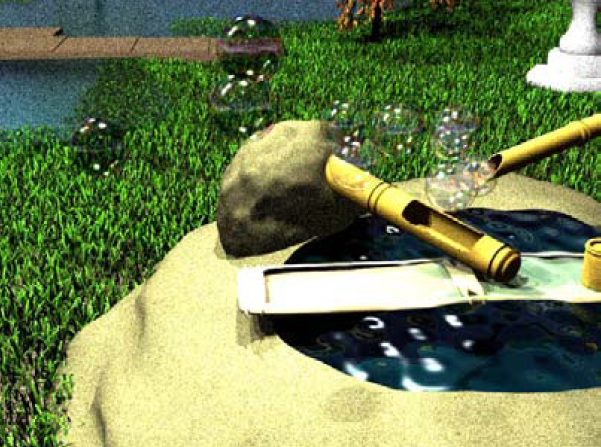
\includegraphics[height=\imageHeight]{images/durikovic/result_animation}
		\caption{Výsledná animácia \cite{durikovic2001}.}
	\end{center}
\end{figure}

Model bublín z tohto článku produkuje fyzikálne veľmi presné bubliny, keďže bubliny sú reprezentované pomocou meshu a sú preto schopné nadobúdať nepravidelné tvary pôsobením rôznych síl. Nevýhodou však je, že táto metóda je výpočtovo náročná a nie je možné pomocou takejto metódy simulovať v reálnom čase penu obsahujúcu stovky bublín a preto takáto metóda nie je vhodná pre implementáciu modelu, ktorý je súčasťou tejto diplomovej práce. V každom prípade z tohto článku môžme využiť v našom modeli niektoré zo síl, ktoré sú v ňom veľmi dobre popísané.

\section{Rendering and Simulation of Liquid Foams \cite{sunkel2004}}

V tomto článku autori prezentujú techniku renderovania a simulácie peny v reálnom čase za pomoci využitia výpočtovej sily GPU. Cieľom bolo vytvoriť model, ktorý by spĺňal fyzikálne vlastnosti interakcie dvoch bublín navzájom a taktiež bublín s inými geometrickými objektmi v scéne ako napr. roviny a dať týmto bublinám realistický vzhľad okrem iného aj za pomoci detailného zobrazenia ich spoločnej steny. Toto všetko dosiahli pomocou dvoch renderovacích fáz. V prvej fáze simulujú interakcie s bublinami a zároveň počítajú spoločné steny medzi každým párom pretínajúcich sa bublín. V druhej fáze sú potom bubliny renderované pomocou shaderov na grafickej karte. Vertex shader dostane informácie o všetkých priesečníkoch medzi bublinami a potom časť vertexov dotýkajúcich sa bublín premiestni do oblasti spoločnej steny týchto bublín. Fragment shader je použitý na vyrátanie osvetlenia pomocou Fresnelovej rovnice.

\subsection{Bubliny}

Cieľom tohto článku je návrh modelu, ktorý je schopný simulovať a renderovať penu v reálnom čase. Avšak najväčším problémom vo virtuálnej realite je renderovanie v reálnom čase. Renderovanie peny je v reálnom čase je obzvlášť náročné použitím štandardných techník. Keďže ľudské oko prehliada niektoré vlastnosti pri pozorovaní pohybujúcich sa objektov, nie je potrebné renderovať fyzikálne presnú penu. Preto sa autori rozhodli pre techniku renderovania peny, ktorá možno nie je fyzikálne úplne presná, ale ľudské oko sa s týmito tvarmi dokáže ľahko stotožniť bez toho, aby si pozorovateľ všimol nejaké fyzikálne nepresnosti. Preto sa autori rozhodli zjednodušiť bubliny a v tomto modeli sú reprezentované ako gule. Ďalším zjednodušením, ktoré autorom ušetrilo veľa problémov a výpočtového času je fakt, že sa rozhodli reprezentovať spoločné steny dotýkajúcich sa bublín len ako rovnú plochu, čo je ďalšia fyzikálna nepresnosť tohto modelu, keďže spoločná stena dvoch bublín je rovná plocha len v prípade, že sa dotýkajú bubliny rovnakej veľkosti, v opačnom prípade je táto stena zaoblená vždy smerom do väčšej bubliny.

\subsection{Simulácia}

Na simuláciu je použitý pružinový systém príťažlivých a odpudivých síl pôsobiacich na bubliny. Príťažlivé sily simulujú vlastnosť minimalizácie povrchového napätia, zatiaľ čo odpudivé sily zabraňujú kolaps navzájom dotýkajúcich sa bublín – má to podobný efekt ako vnútorný tlak, ktorý pôsobí na vnútornú stenu bubliny. Tieto dve sily (príťažlivá a odpudivá) sú navzájom konkurenčné a zabezpečujú stabilitu systému, ktorá je podobná stabilite, ktorú zabezpečujú Plateauové pravidlá. Odpudivá sila $F_{ij}^{r}$ pôsobiaca na bublinu $i$ vzhľadom na jej kontakt s bublinou $j$ je definovaná takto:
\begin{equation}
	F_{ij}^{r}=k_{r}\left(\frac{1}{\parallel p_{i} - p_{j} \parallel} - \frac{1}{rad_{i} + rad_{j}}\right) \left(p_i - p_j\right), 
\end{equation}
kde \textit{k\sub{r}} je používateľom definovaná konštanta povrchového napätia kvapaliny. Príťažlivá sila \textit{$F_{ij}^{a}$} medzi dvomi bublinami \textit{i, j} závisí od veľkosti povrchu, ktorý tieto bubliny zdieľajú a platí, že čím viac sa dotýkajú, tým je táto sila menšia. Rovnica tejto sily vyzerá nasledovne:
\begin{equation}
	F_{ij}^{a} = k_{a}c_{nb}c_{dist}\frac{p_{j} - p_{i}}{\parallel p_{j} - p_{i}\parallel},
\end{equation}
kde
\begin{equation}
	c_{nb} = \frac{\frac{1}{\left | NB_{i} \right |} + \frac{1}{\left | NB_{j} \right |}}{2},\qquad c_{dist} = \frac{\left \| p_{j} - p_{i} \right \| - max(rad_{i}, rad_{j})}{min(rad_{i}, rad_{j})}.
\end{equation}
Opäť \textit{k\sub{a}} je používateľom definovaný koeficient tak, že \textit{k\sub{a}/k\sub{r}} tvoria vlhkosť simulovanej peny. $\left | NB_{i} \right |$ je počet susedných bublín dotýkajúcich sa alebo pretínajúcich bublinu \textit{i}. Okrem týchto síl v tomto modeli využívajú aj ďalšie sily ako napr. odpor vzduchu a takisto príťažlivé a odpudivé sily vzhľadom na objekty.

\subsection{Programy zbiehajúce na grafickej karte}

Asi najzaujímavejšou časťou tohto článku je riešenie zobrazovania spoločnej steny medzi bublinami. Nakoľko počas počítania simulácie sa ukladá o každej spoločnej rovine iba informácia o jej normálovej forme rovnice roviny a s bublinami sa pri výpočtoch pracuje ako s guľami, autori museli vymyslieť spôsob, ako tieto dotýkajúce sa gule orezať. Práve na toto využili výpočtovú silu GPU a použili na to program zbiehajúci na grafickej karte, tzv. vertex shader. Do vertex shadera sa najprv pošlú vertexy na povrchu každej z gulí a následne je vertex shader naplnený pretínajúcimi rovinami $e_{i}: n_{i}x - d_{i} = 0$. Pretínajúce roviny sa počítajú na začiatku každého snímku. Na obrázku \reference{img:cross_section_of_two_spheres} vidieť pretínajúcu sa oblasť dvoch gúľ:
\begin{figure}[H]
	\begin{center}
		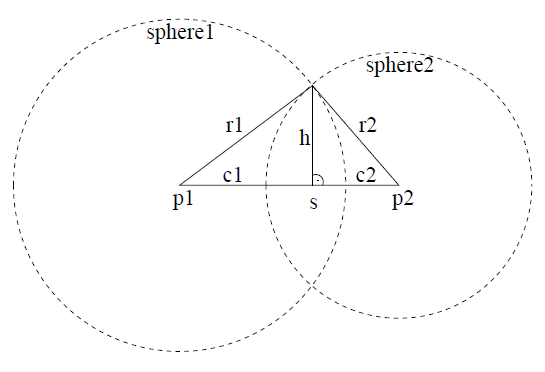
\includegraphics[height=\imageHeight]{images/sunkel/cross_section_of_two_spheres}
		\caption{Spoločná rovina dvoch gúľ \cite{sunkel2004}.}
		\label{img:cross_section_of_two_spheres}
	\end{center}
\end{figure}
\noindent Zo súradnicového systému gule 1 potom dostávame rovnicu:
\begin{equation}
	\label{eq:sunkel:s}
	s = c_{1}.n,
\end{equation}
kde
\begin{equation}
	\label{eq:sunkel:c1_n}
	c_{1} = \frac{r_{1}^{2} - r_{2}^{2} + d^{2}}{2d}, \qquad n = \frac{p_{2} - p_{1}}{\left \| p_{2} - p_{1} \right \|} = \frac{p_{2} - p_{1}}{d}.
\end{equation}
Teda rovnica spoločnej roviny medzi guľou 1 a guľou 2 vyzerá nasledovne:
\begin{equation}
	\label{eq:sunkel:common_plane}
	e: \frac{p_{2} - p_{1}}{d}\ast x - \frac{r_{1}^{2} - r_{2}^{2} + d^{2}}{2d} = 0.
\end{equation}
Vertex shader potom presunie vertexy gulí do spoločnej roviny. Výber vertexov, ktoré je potrebné z každej gule posunúť funguje nasledovne: pre všetky vertexy \textit{p\sub{i}} gule a pre všetky spoločné steny $e_{j}: n_{j}x - d_{j} = 0$ vertex shader vypočíta
\begin{equation}
	\label{eq:sunkel:lambda}
	\lambda _{ij} = d_{j} - n_{j}\cdot p_{i},
\end{equation}
a v prípade, že $\lambda _{ij} < 0$, tak bod $p_{i}$ nahradí nasledovne:
\begin{equation}
	\label{eq:sunkel:vertex_displacement}
	p_{i} := p_{i} + \lambda _{ij} \cdot n_{j}.
\end{equation}
Na obrázku \reference{img:verticies_displacement} a \reference{img:verticies_displacement_2} vidieť akým spôsobom sú vertexy nahradené.
\begin{figure}[H]
	\begin{center}
		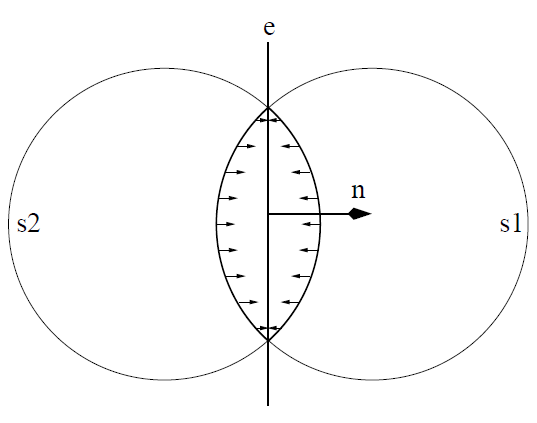
\includegraphics[height=\imageHeight]{images/sunkel/verticies_displacement}
		\caption{Premiestňovanie vertexov na spoločnú stenu gúľ \cite{sunkel2004}.}
		\label{img:verticies_displacement}
	\end{center}
\end{figure}
\begin{figure}[H]
	\begin{center}
		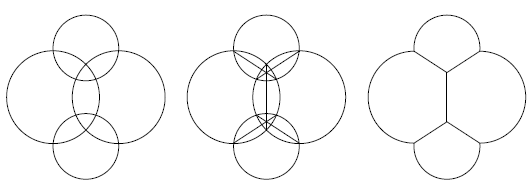
\includegraphics[width=\textwidth]{images/sunkel/verticies_displacement_2}
		\caption{Premiestňovanie vertexov na spoločné steny pri kolízií viacerých gúľ \cite{sunkel2004}.}
		\label{img:verticies_displacement_2}
	\end{center}
\end{figure}

\subsection{Diskusia}

Finálna simulácia, ktorú spravili, obsahovala okolo 21 rovín, s ktorými mohli bubliny kolidovať a obsahovala bubliny, ktoré mali náhodne generovanú ako veľkosť, tak aj pozíciu. Hoci v tomto štádiu nespĺňali fyzikálne vlastnosti peny tohto modelu, po prvom simulačnom kroku sa dostali do stabilného rozpoloženia, t.j. rovnováhy medzi príťažlivými a odpudivými silami. Táto simulácia bežala na procesore Intel XEON 1.7GHz a na grafickej karte GeForceFX 5800 pri 10 fps.
\begin{figure}[H]
	\begin{center}
		\includegraphics[width=\textwidth]{images/sunkel/results}
		\caption{Výsledná animácia \cite{sunkel2004}.}
	\end{center}
\end{figure}

Z tejto práce je asi najzaujímavejšie riešenie, akým docielili orezávanie dotýkajúcich sa bublín a je to určite jedna z vecí, ktorú by sme mohli využiť pri tvorbe nášho modelu.

\section{Animating Bubble Interactions in a Liquid Foam \cite{busaryev2012}}

Tento článok popisuje model na simuláciu peny, ktorý sa zameriava najmä na to simuláciu a vizualizáciu peny s malými bublinami, ktorých polomer je menší ako 1 cm. Keďže bubliny takejto malej veľkosti sú oveľa viac ovplyvnené povrchovým napätím v porovnaní s veľkými bublinami, sú preto oveľa menej deformovateľné a tak je ich tvar takmer vždy guľovitý. Preto sa autori rozhodli použiť časticový systém, ktorého častice (bubliny) sú gule. Autori navrhli efektívny algoritmus pre takýto časticový systém, ktorého kľúčovým prvkom je aproximácia geometrie peny použitím váženého Voronoiovho diagramu. Použitím Voronoiových buniek a váh je možné takisto explicitne zistiť problém straty objemu jednotlivých bublín, čo bol spoločný problém viacerých predchádzajúcich riešení.

\subsection{Pena a bubliny}

V tomto modeli je zanedbaná deformácia jednotlivých bublín a tak má každá bublina pravidelný guľovitý tvar. Pena ako celok je vlastne rozdelenie priestoru medzi gule. Autori sa preto rozhodli použiť na reprezentáciu peny dátovú štruktúru nazývanú space-filling diagram, ktorá rozdeľuje priestor rovnakým spôsobom. Space-filling diagram je priesečník zjednotenia gúl s váženým Voronoiovým diagramom. V takejto dátovej štruktúre je bublina $B_{i} = B(x_{i}, r_{i})$ reprezentovaná ako priesečník medzi $B_{i}$ a bunkou $x_{i}$ s váhou $r_{i}$ z váženého Voronoiovho diagramu. Na nasledujúcom obrázku vidieť dátovú štruktúru takto reprezentovanej peny.
\begin{figure}[H]
	\begin{center}
		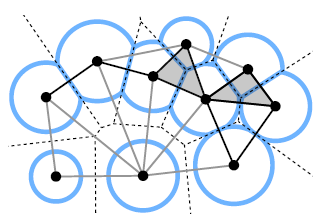
\includegraphics[height=100px]{images/busaryev/foam_voronoi_space_filling}
		\caption{Štruktúra peny \cite{busaryev2012}.}
	\end{center}
\end{figure}

\subsection{Dynamika peny}

Pri dynamike peny sa autori venovali trom typom interakcie bublín: interakcia medzi bublinami navzájom, interakcia medzi bublinami a tekutinou a interakcia medzi bublinami a tuhým telesom. Keďže v modeli, ktorý je súčasťou tejto diplomovej práce sa budem venovať primárne interakcii medzi bublinami navzájom, budem z tohto článku ďalej rozoberať iba tento typ interakcie. Na simuláciu interakcie medzi dvomi dotýkajúcimi bublinami je v tomto modeli použitý pružinový systém, podobne ako v modeloch od Kück a spol. z roku 2002, resp. Greenwood a House z roku 2004. Nech $x_{i}$ a $x_{j}$ sú stredy dotýkajúcich sa bublín, potom interakčná sila pôsobiaca na xi použitím pokojovej dĺžky $l_{ij}$ vyzerá nasledovne:
\begin{equation}
	f_{i}^{sint} = -k\sum_{j}\left ( x_{i} - x_{j} - l_{ij} \frac{x_{i} - x_{j}}{\left | x_{i} - x_{j} \right |} \right ),
\end{equation}
kde \textit{k} je koeficient tuhosti.

\subsection{Simulácia peny}

Na simuláciu vyvinuli simulátor peny, ktorý upravuje bubliny peny v každom časovom kroku. Na začiatku využíva implicitný integrátor na získanie pozície a rýchlosti jednotlivých bublín vzhľadom na dynamiku peny. Následne je použitá technika na zachovanie objemu bublín, ktorá kompenzuje stratu objemu bublín počas simulácie. Na záver tento simulátor vykoná topologické zmeny štruktúry peny a rekonštruuje vážený Voronoiov diagram tak, aby zabezpečil korektnosť tohto diagramu pre ďalší simulačný krok. Časový integrátor využíva na riešenie vývoju častíc implicitnú metódu, ktorú navrhli Baraff a Witkin v roku 1998. Vzhľadom na pozície bublín ${x_{i}^{t}}$ a ich rýchlosti ${v_{i}^{t}}$ v čase \textit{t}, je na riešenie použitá spätná Eulerová metóda, pomocou ktorej sa vypočítajú rýchlosti bublín ${v_{i}^{t+1}}$ ďalšom časovom kroku:
\begin{equation}
	\left ( M - \Delta t\partial f^{t}/\partial v - \Delta t^{2}\partial f^{t}/\partial x \right )v^{t+1} = Mv^{t} + \Delta tf^{t},
\end{equation}
kde \textit{M} je matica váh, $\Delta t$ je časový krok a $f, x$ a $v$ sú vektory síl, pozícií a rýchlosti bublín. Vektor $f$ je súčtom gravitačnej sily, odporu vzduchu a celkovej interakčnej sily. Tento lineárny systém riešili pomocou PCG metódy. Keďže interakčné sily sú závislé na spojitosti jednotlivých bublín, ktorá sa môže meniť v čase, tento systém nemusí byť bezpodmienečne stabilný. Experimenty však ukázali, že systém zvládal simulovať penu aj pri veľkých časových krokoch ($\Delta t\;\in\;[0.005s, 0.02s]$) pri väčšine testovaných príkladov.

\subsection{Diskusia}

Táto práca je založená na pružinovom systéme, ktorý tu je dobre popísaný a mohli by sme sa ním inšpirovať pri tvorbe nášho modelu.
\begin{figure}[H]
	\begin{center}
		\includegraphics[height=\imageHeight]{images/busaryev/results}
		\caption{Výsledná animácia \cite{busaryev2012}.}
	\end{center}
\end{figure}